\documentclass[12pt,a4paper]{article}

% Packages
\usepackage[utf8]{inputenc}
\usepackage[english]{babel}
\usepackage{amsmath,amssymb,amsthm}
\usepackage{graphicx}
\usepackage{geometry}
\usepackage{float}
\usepackage{caption}
\usepackage{subcaption}
\usepackage{hyperref}
\usepackage{siunitx}
\usepackage{booktabs}
\usepackage{bm}
\usepackage{pdfpages}

% Page geometry
\geometry{margin=2.5cm}

% Custom commands
\newcommand{\parder}[2]{\frac{\partial #1}{\partial #2}}
\newcommand{\pparder}[2]{\frac{\partial^2 #1}{\partial #2^2}}
\newcommand{\Rey}{\text{Re}}
\newcommand{\Pran}{\text{Pr}}

\begin{document}

% Title page
\begin{titlepage}
    \centering
    \vspace*{2cm}

    {\Huge\bfseries Development of Flow at the Entrance of a Cylindrical Pipe\par}

    \vspace{1.5cm}

    {\Large Numerical Simulation and Modelling of Incompressible Flow\par}

    \vspace{1cm}

    {\large LV-Nr.: 321.053 EX\par}
    {\large Winter Semester 2025/26\par}

    \vfill

    {\Large
    Felix Scope\\
    \texttt{felix\_scope@yahoo.de}\\
    }

    \vfill

    {\large \today\par}
\end{titlepage}

\tableofcontents
\newpage

% Include the assignment (as per guidelines)
\section*{Assignment}
\addcontentsline{toc}{section}{Assignment}
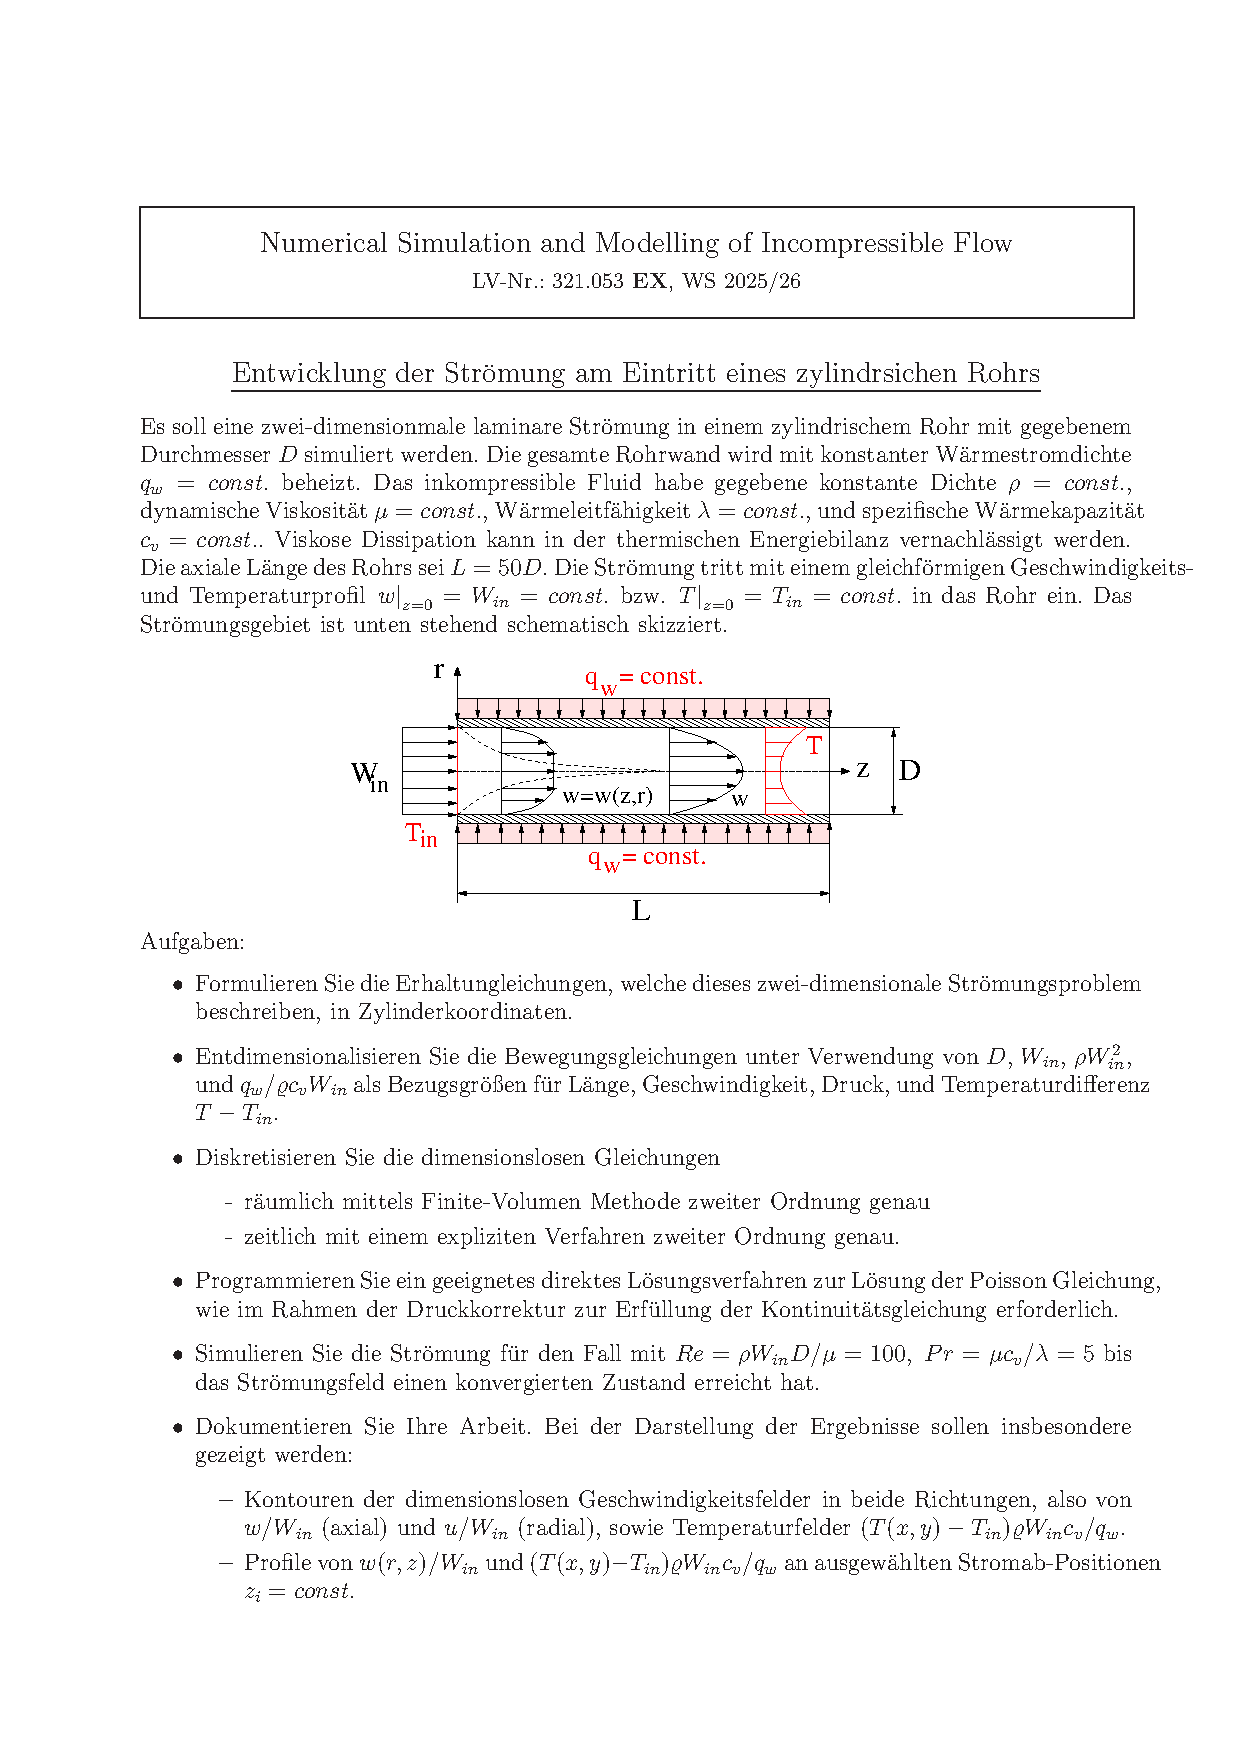
\includepdf[pages=-]{../Assignemnt/Assignment_WS25.pdf}

\newpage

\section{Problem Description}

\subsection{Geometry and Setup}

The problem considers a two-dimensional laminar flow in a cylindrical pipe with diameter $D$ and length $L = 50D$. The entire pipe wall is heated with constant heat flux $q_w = \text{const.}$ The incompressible fluid has constant properties: density $\rho$, dynamic viscosity $\mu$, thermal conductivity $\lambda$, and specific heat capacity $c_v$. Viscous dissipation is neglected in the thermal energy balance.

The flow enters the pipe with uniform velocity and temperature profiles:
\begin{align}
    w\big|_{z=0} &= W_{\text{in}} = \text{const.} \\
    T\big|_{z=0} &= T_{\text{in}} = \text{const.}
\end{align}

The computational domain is shown schematically in Figure~\ref{fig:geometry}.

\begin{figure}[H]
    \centering
    
\includegraphics[width=0.95\textwidth]{../Plots_python/geometry_diagram.png}
    \caption{Schematic of the cylindrical pipe flow with constant wall heat flux. Flow enters with uniform velocity $W_{\text{in}}$ and temperature $T_{\text{in}}$, and develops into a parabolic profile along the pipe length.}
    \label{fig:geometry}
\end{figure}

\subsection{Physical Parameters}

\begin{itemize}
    \item Reynolds number: $\Rey = \frac{\rho W_{\text{in}} D}{\mu} = 100$
    \item Prandtl number: $\Pran = \frac{\mu c_v}{\lambda} = 5$
    \item Length-to-diameter ratio: $L/D = 50$
\end{itemize}

\newpage

\section{Mathematical Formulation}

\subsection{Governing Equations in Cylindrical Coordinates}

For an axisymmetric flow in cylindrical coordinates $(r, z)$ with velocity components $(u, w)$ in the radial and axial directions respectively, the governing equations are:

\subsubsection{Continuity Equation}

The continuity equation for an incompressible fluid is:
\begin{equation}
    \parder{u}{r} + \frac{u}{r} + \parder{w}{z} = 0
    \label{eq:continuity_dim}
\end{equation}

\subsubsection{Momentum Equations}

The Navier-Stokes equations in cylindrical coordinates for axisymmetric flow are:

\textbf{Radial momentum:}
\begin{equation}
    \parder{u}{t} + u\parder{u}{r} + w\parder{u}{z} = -\frac{1}{\rho}\parder{p}{r} + \nu\left(\pparder{u}{r} + \frac{1}{r}\parder{u}{r} - \frac{u}{r^2} + \pparder{u}{z}\right)
    \label{eq:momentum_r_dim}
\end{equation}

\textbf{Axial momentum:}
\begin{equation}
    \parder{w}{t} + u\parder{w}{r} + w\parder{w}{z} = -\frac{1}{\rho}\parder{p}{z} + \nu\left(\pparder{w}{r} + \frac{1}{r}\parder{w}{r} + \pparder{w}{z}\right)
    \label{eq:momentum_z_dim}
\end{equation}

where $\nu = \mu/\rho$ is the kinematic viscosity.

\subsubsection{Energy Equation}

The energy equation (neglecting viscous dissipation) is:
\begin{equation}
    \parder{T}{t} + u\parder{T}{r} + w\parder{T}{z} = \alpha\left(\pparder{T}{r} + \frac{1}{r}\parder{T}{r} + \pparder{T}{z}\right)
    \label{eq:energy_dim}
\end{equation}

where $\alpha = \lambda/(\rho c_v)$ is the thermal diffusivity.

\subsection{Boundary Conditions}

\textbf{Inlet} ($z = 0$):
\begin{align}
    u(r, 0) &= 0 \\
    w(r, 0) &= W_{\text{in}} \\
    T(r, 0) &= T_{\text{in}}
\end{align}

\textbf{Wall} ($r = D/2$):
\begin{align}
    u(D/2, z) &= 0 \\
    w(D/2, z) &= 0 \\
    -\lambda\parder{T}{r}\bigg|_{r=D/2} &= q_w
\end{align}

\textbf{Centerline} ($r = 0$, symmetry):
\begin{align}
    \parder{u}{r}\bigg|_{r=0} &= 0 \quad \text{(or } u(0,z) = 0\text{)}\\
    \parder{w}{r}\bigg|_{r=0} &= 0 \\
    \parder{T}{r}\bigg|_{r=0} &= 0
\end{align}

\textbf{Outlet} ($z = L$):
\begin{equation}
    \parder{u}{z}\bigg|_{z=L} = 0, \quad \parder{w}{z}\bigg|_{z=L} = 0, \quad \parder{T}{z}\bigg|_{z=L} = 0
\end{equation}

\newpage

\section{Non-Dimensionalization}

\subsection{Reference Scales}

We introduce the following reference scales:
\begin{itemize}
    \item Length: $D$
    \item Velocity: $W_{\text{in}}$
    \item Pressure: $\rho W_{\text{in}}^2$
    \item Temperature difference: $\frac{q_w}{\rho c_v W_{\text{in}}}$
\end{itemize}

\subsection{Non-Dimensional Variables}

Define the non-dimensional variables (denoted with asterisks):
\begin{align}
    r^* &= \frac{r}{D}, \quad z^* = \frac{z}{D} \\
    u^* &= \frac{u}{W_{\text{in}}}, \quad w^* = \frac{w}{W_{\text{in}}} \\
    p^* &= \frac{p}{\rho W_{\text{in}}^2} \\
    \theta &= \frac{(T - T_{\text{in}})\rho c_v W_{\text{in}}}{q_w} \\
    t^* &= \frac{t W_{\text{in}}}{D}
\end{align}

\subsection{Non-Dimensional Governing Equations}

Substituting the non-dimensional variables into equations~\eqref{eq:continuity_dim}--\eqref{eq:energy_dim} yields:

\subsubsection{Non-Dimensional Continuity}
\begin{equation}
    \parder{u^*}{r^*} + \frac{u^*}{r^*} + \parder{w^*}{z^*} = 0
    \label{eq:continuity_nondim}
\end{equation}

\subsubsection{Non-Dimensional Momentum Equations}

\textbf{Radial momentum:}
\begin{equation}
    \parder{u^*}{t^*} + u^*\parder{u^*}{r^*} + w^*\parder{u^*}{z^*} = -\parder{p^*}{r^*} + \frac{1}{\Rey}\left(\pparder{u^*}{r^*} + \frac{1}{r^*}\parder{u^*}{r^*} - \frac{u^*}{r^{*2}} + \pparder{u^*}{z^*}\right)
    \label{eq:momentum_r_nondim}
\end{equation}

\textbf{Axial momentum:}
\begin{equation}
    \parder{w^*}{t^*} + u^*\parder{w^*}{r^*} + w^*\parder{w^*}{z^*} = -\parder{p^*}{z^*} + \frac{1}{\Rey}\left(\pparder{w^*}{r^*} + \frac{1}{r^*}\parder{w^*}{r^*} + \pparder{w^*}{z^*}\right)
    \label{eq:momentum_z_nondim}
\end{equation}

\subsubsection{Non-Dimensional Energy Equation}

\begin{equation}
    \parder{\theta}{t^*} + u^*\parder{\theta}{r^*} + w^*\parder{\theta}{z^*} = \frac{1}{\Rey\Pran}\left(\pparder{\theta}{r^*} + \frac{1}{r^*}\parder{\theta}{r^*} + \pparder{\theta}{z^*}\right)
    \label{eq:energy_nondim}
\end{equation}

\subsection{Non-Dimensional Boundary Conditions}

\textbf{Inlet} ($z^* = 0$):
\begin{equation}
    u^* = 0, \quad w^* = 1, \quad \theta = 0
\end{equation}

\textbf{Wall} ($r^* = 1/2$):
\begin{equation}
    u^* = 0, \quad w^* = 0, \quad \parder{\theta}{r^*} = -1
\end{equation}

\textbf{Centerline} ($r^* = 0$):
\begin{equation}
    \parder{u^*}{r^*} = 0 \text{ (or } u^* = 0\text{)}, \quad \parder{w^*}{r^*} = 0, \quad \parder{\theta}{r^*} = 0
\end{equation}

\textbf{Outlet} ($z^* = L/D = 50$):
\begin{equation}
    \parder{u^*}{z^*} = 0, \quad \parder{w^*}{z^*} = 0, \quad \parder{\theta}{z^*} = 0
\end{equation}

\newpage

\section{Numerical Solution}

\subsection{Computational Domain}

The computational domain is rectangular in the $(r^*, z^*)$ plane:
\begin{equation}
    \Omega = \{(r^*, z^*) : 0 \leq r^* \leq 0.5, \quad 0 \leq z^* \leq 50\}
\end{equation}

\subsection{Grid Structure}

A staggered grid arrangement is employed:
\begin{itemize}
    \item \textbf{Scalar variables} ($p^*$, $\theta$): stored at cell centers
    \item \textbf{Velocity components}: stored at cell faces
    \begin{itemize}
        \item $u^*$: stored at radial faces (between cells in $r$-direction)
        \item $w^*$: stored at axial faces (between cells in $z$-direction)
    \end{itemize}
\end{itemize}

Grid parameters:
\begin{itemize}
    \item Number of cells in radial direction: $n_r$
    \item Number of cells in axial direction: $n_z$
    \item Uniform grid spacing: $\Delta r^* = 0.5/n_r$, $\Delta z^* = 50/n_z$
\end{itemize}

\subsection{Spatial Discretization}

The governing equations are discretized using the \textbf{Finite Volume Method} with \textbf{second-order accuracy}.

\subsubsection{Continuity Equation Discretization}

Integrating equation~\eqref{eq:continuity_nondim} over a control volume and applying Gauss divergence theorem:
\begin{equation}
    \left[\frac{(r^*u^*)_e - (r^*u^*)_w}{r^*_P\Delta r^*}\right] + \left[\frac{w^*_n - w^*_s}{\Delta z^*}\right] = 0
\end{equation}

where subscripts $e, w, n, s$ denote east, west, north, south faces, and $P$ denotes the cell center.

\subsubsection{Convection-Diffusion Discretization}

For the momentum and energy equations, we discretize the convective and diffusive terms:

\textbf{Convective terms} (second-order central differencing):
\begin{equation}
    u^*\parder{\phi}{r^*} \approx u^*_e\frac{\phi_E - \phi_P}{\Delta r^*}
\end{equation}

\textbf{Diffusive terms} (second-order central differencing):
\begin{equation}
    \pparder{\phi}{r^*} \approx \frac{\phi_E - 2\phi_P + \phi_W}{(\Delta r^*)^2}
\end{equation}

\subsection{Temporal Discretization}

A second-order explicit time integration scheme is employed (e.g., second-order Adams-Bashforth or Runge-Kutta RK2).

For a generic transport equation:
\begin{equation}
    \parder{\phi}{t^*} = F(\phi)
\end{equation}

\textbf{Second-order Adams-Bashforth:}
\begin{equation}
    \phi^{n+1} = \phi^n + \Delta t^*\left[\frac{3}{2}F(\phi^n) - \frac{1}{2}F(\phi^{n-1})\right]
\end{equation}

\subsection{Pressure Correction Method}

A segregated solution approach based on the \textbf{projection method} with pressure correction is used:

\begin{enumerate}
    \item \textbf{Predictor step}: Solve momentum equations without pressure gradient to obtain intermediate velocities $u^{**}, w^{**}$

    \item \textbf{Pressure correction}: Solve the Poisson equation for pressure correction $p'$:
    \begin{equation}
        \nabla^2 p' = \frac{\rho}{\Delta t}\nabla \cdot \bm{u}^{**}
        \label{eq:poisson}
    \end{equation}

    In non-dimensional form:
    \begin{equation}
        \pparder{p'}{r^{*2}} + \frac{1}{r^*}\parder{p'}{r^*} + \pparder{p'}{z^{*2}} = \frac{1}{\Delta t^*}\left(\parder{u^{**}}{r^*} + \frac{u^{**}}{r^*} + \parder{w^{**}}{z^*}\right)
    \end{equation}

    \item \textbf{Velocity correction}:
    \begin{align}
        u^{n+1} &= u^{**} - \Delta t^*\parder{p'}{r^*} \\
        w^{n+1} &= w^{**} - \Delta t^*\parder{p'}{z^*}
    \end{align}

    \item \textbf{Pressure update}:
    \begin{equation}
        p^{n+1} = p^n + \alpha_p p'
    \end{equation}
    where $\alpha_p$ is an under-relaxation factor.
\end{enumerate}

\subsection{Poisson Solver}

The Poisson equation~\eqref{eq:poisson} is solved using a direct solver. For cylindrical coordinates, the discretized Poisson equation yields a banded linear system:
\begin{equation}
    \mathbf{A}\mathbf{p}' = \mathbf{b}
\end{equation}

This system is solved using:
\begin{itemize}
    \item \textbf{Direct method}: LU decomposition or Cholesky decomposition for banded matrices
    \item \textbf{Iterative method}: Successive Over-Relaxation (SOR) or Conjugate Gradient
\end{itemize}

\newpage

\section{Analytical Solution}

For fully developed flow (at large $z^*$), analytical solutions exist:

\subsection{Velocity Profile}

The fully developed velocity profile is parabolic (Hagen-Poiseuille flow):
\begin{equation}
    \frac{w}{W_{\text{in}}} = 2\left[1 - \left(\frac{2r}{D}\right)^2\right] = 2\left[1 - (2r^*)^2\right]
    \label{eq:analytical_velocity}
\end{equation}

The centerline velocity is:
\begin{equation}
    w_{\text{max}} = 2W_{\text{in}}
\end{equation}

\subsection{Temperature Profile}

The fully developed temperature profile for constant wall heat flux:
\begin{equation}
    \theta = \frac{(T - T_{\text{in}})\rho c_v W_{\text{in}}}{q_w} = 4\frac{z}{D} + \Rey\Pran\left[\left(\frac{2r}{D}\right)^2 - \frac{1}{4}\left(\frac{2r}{D}\right)^4 - \frac{3}{4}\right]
    \label{eq:analytical_temperature}
\end{equation}

or in non-dimensional form:
\begin{equation}
    \theta = 4z^* + \Rey\Pran\left[(2r^*)^2 - \frac{1}{4}(2r^*)^4 - \frac{3}{4}\right]
\end{equation}

\subsection{Nusselt Number}

For fully developed thermal flow with constant wall heat flux (H1 boundary condition):
\begin{equation}
    \text{Nu} = \frac{48}{11} \approx 4.364
\end{equation}

\newpage

\section{Results}

\subsection{Convergence Criteria}

The simulation is run until convergence is achieved. Convergence is monitored using residuals:

\textbf{Continuity residual:}
\begin{equation}
    R_{\text{cont}} = \max_{i,j}\left|\parder{u^*}{r^*} + \frac{u^*}{r^*} + \parder{w^*}{z^*}\right|_{i,j}
\end{equation}

\textbf{Velocity residual:}
\begin{equation}
    R_{\text{vel}} = \max\left(\frac{\|u^{n+1} - u^n\|}{\Delta t}, \frac{\|w^{n+1} - w^n\|}{\Delta t}\right)
\end{equation}

\textbf{Temperature residual:}
\begin{equation}
    R_{\text{temp}} = \frac{\|\theta^{n+1} - \theta^n\|}{\Delta t}
\end{equation}

Convergence is declared when:
\begin{equation}
    R_{\text{cont}} < 10^{-6}, \quad R_{\text{vel}} < 10^{-6}, \quad R_{\text{temp}} < 10^{-6}
\end{equation}

\subsection{Expected Results}

The following results will be presented:

\begin{enumerate}
    \item \textbf{Velocity field contours}: $w^*(r^*, z^*)$ and $u^*(r^*, z^*)$
    \item \textbf{Temperature field contours}: $\theta(r^*, z^*)$
    \item \textbf{Velocity profiles}: $w^*(r^*)$ at selected axial positions $z^* = \{5, 10, 20, 30, 40, 50\}$
    \item \textbf{Temperature profiles}: $\theta(r^*)$ at selected axial positions
    \item \textbf{Comparison with analytical solutions}: Equations~\eqref{eq:analytical_velocity} and~\eqref{eq:analytical_temperature}
    \item \textbf{Convergence history}: Plot of residuals vs. iteration/time step
\end{enumerate}

\section{Conclusion}

This report presents the mathematical formulation, non-dimensionalization, and numerical solution strategy for simulating the developing flow in a heated cylindrical pipe. The finite volume method with second-order spatial and temporal discretization is employed, along with a pressure correction method for enforcing the continuity constraint. The Poisson equation for pressure correction is solved using a direct solver. Results will be validated against analytical solutions for fully developed flow.

\end{document}
